% Created 2021-04-13 Tue 13:08
% Intended LaTeX compiler: pdflatex
\documentclass[11pt]{article}
\usepackage[utf8]{inputenc}
\usepackage[T1]{fontenc}
\usepackage{graphicx}
\usepackage{grffile}
\usepackage{longtable}
\usepackage{wrapfig}
\usepackage{rotating}
\usepackage[normalem]{ulem}
\usepackage{amsmath}
\usepackage{textcomp}
\usepackage{amssymb}
\usepackage{capt-of}
\usepackage{hyperref}
\usepackage[a4paper, lmargin=25mm, rmargin=25mm, tmargin=25mm, bmargin=25mm]{geometry}
\date{2021 April 13}
\title{TAB2XML User Manual\\\medskip
\large For Version 1.0.0}
\hypersetup{
 pdfauthor={},
 pdftitle={TAB2XML User Manual},
 pdfkeywords={},
 pdfsubject={},
 pdfcreator={Emacs 27.1 (Org mode 9.4.4)}, 
 pdflang={English}}
\begin{document}

\maketitle
\tableofcontents

\newpage

\section{Introduction and Purpose}
\label{sec:orgbdd28ce}
The TAB2XML system can be used to convert text tablature into MusicXML.  This document outlines how to install and use the system in many use cases.
\section{System Requirements}
\label{sec:org152fbb0}
\begin{itemize}
\item Works on all major operating systems
\item Java version 11-15 required
\end{itemize}
\section{How to Install TAB2XML}
\label{sec:org56b0587}
\subsection{Eclipse}
\label{sec:orge0886ee}
\begin{enumerate}
\item Open Eclipse, and press \texttt{File > Import} in the menus.
\begin{center}
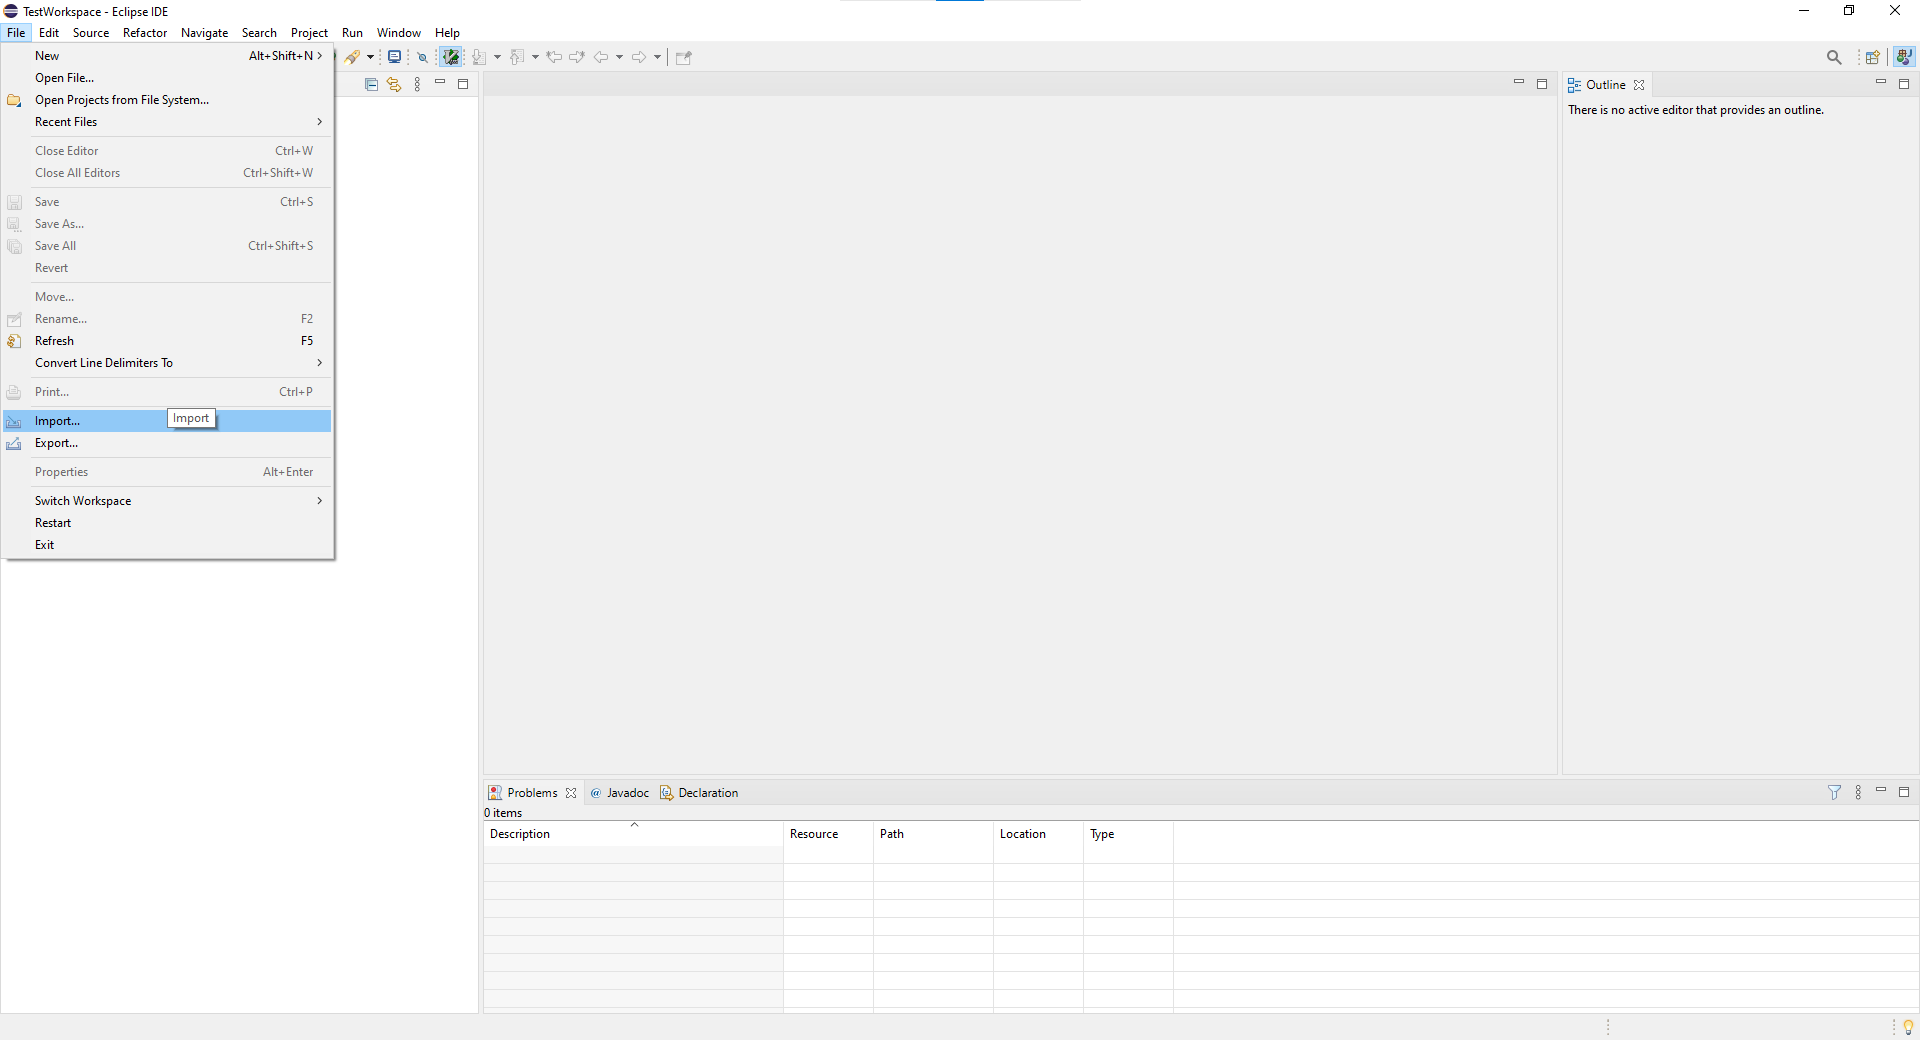
\includegraphics[width=.9\linewidth]{../Screenshots/eclipse-install-1.png}
\end{center}
\item In the window that opens, select "Projects from Git", in the folder called "Git".  Then, click "Next"
\begin{center}
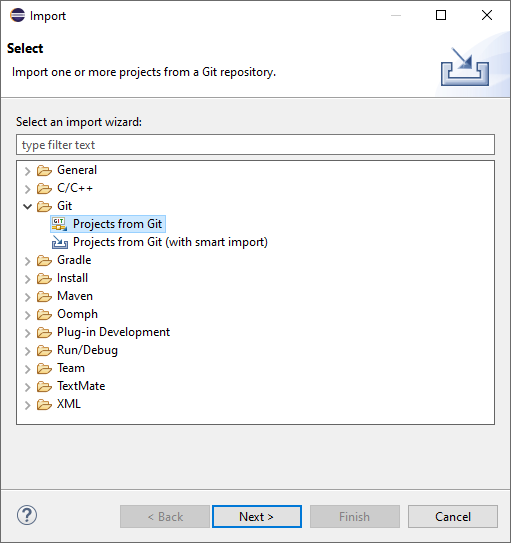
\includegraphics[width=.9\linewidth]{../Screenshots/eclipse-install-2.png}
\end{center}
\item Click "Clone URI" then click "Next".
\begin{center}
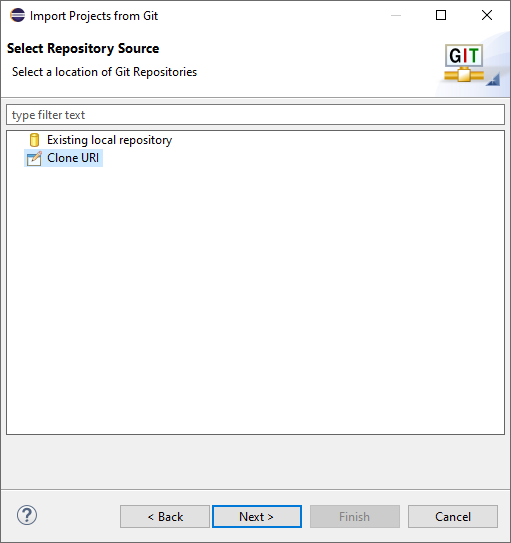
\includegraphics[width=.9\linewidth]{../Screenshots/eclipse-install-3.png}
\end{center}
\item Enter "\texttt{https://github.com/ahopk127/eecs2311-tab2xml.git}" in the first field ("URI"), then click "Next".  No authentication is required.
\begin{center}
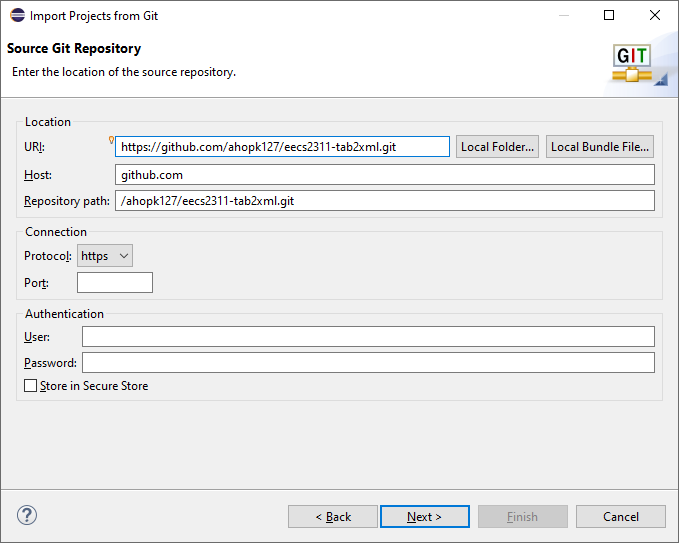
\includegraphics[width=.9\linewidth]{../Screenshots/eclipse-install-4.png}
\end{center}
\item Choose where you want the program to be saved on your computer (or just use the default location), then click "Next".
\begin{center}
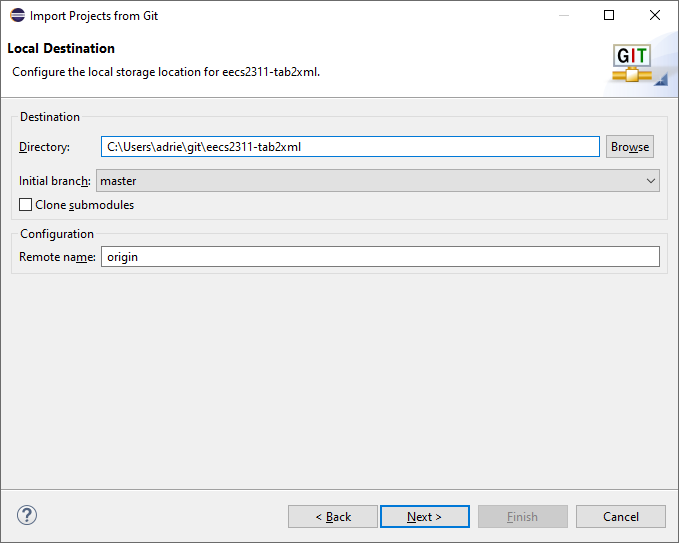
\includegraphics[width=.9\linewidth]{../Screenshots/eclipse-install-5.png}
\end{center}
\item Click "Next" then "Finish".  The program is now installed on your computer, but must be built using Gradle.
\begin{center}
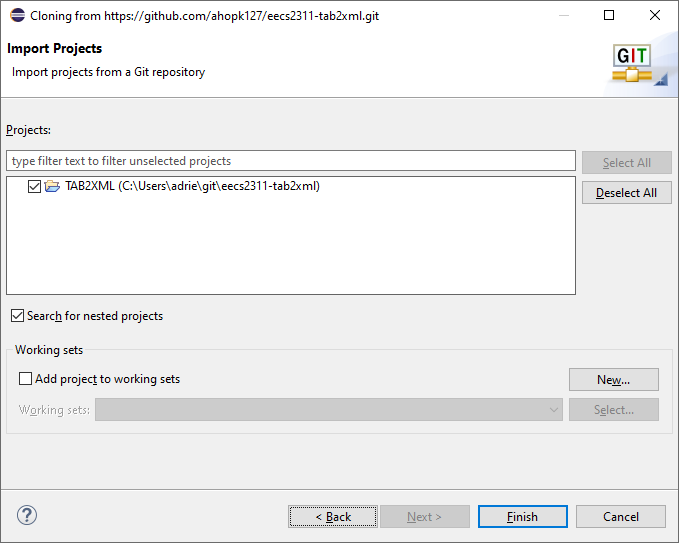
\includegraphics[width=.9\linewidth]{../Screenshots/eclipse-install-7.png}
\end{center}
\item You will need the "Gradle Tasks" window for the next step.  If you can't find it, press \texttt{Window > Show View > Other} in the menu, then find "Gradle Tasks" in the Gradle folder, then click "Open".
\begin{center}
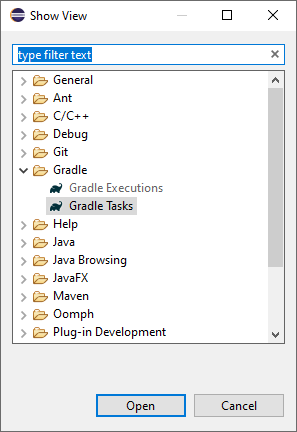
\includegraphics[width=.9\linewidth]{../Screenshots/eclipse-build-2.png}
\end{center}
\item In the "Gradle Tasks" window, double-click the green "build" item in the "build" folder.
\begin{center}
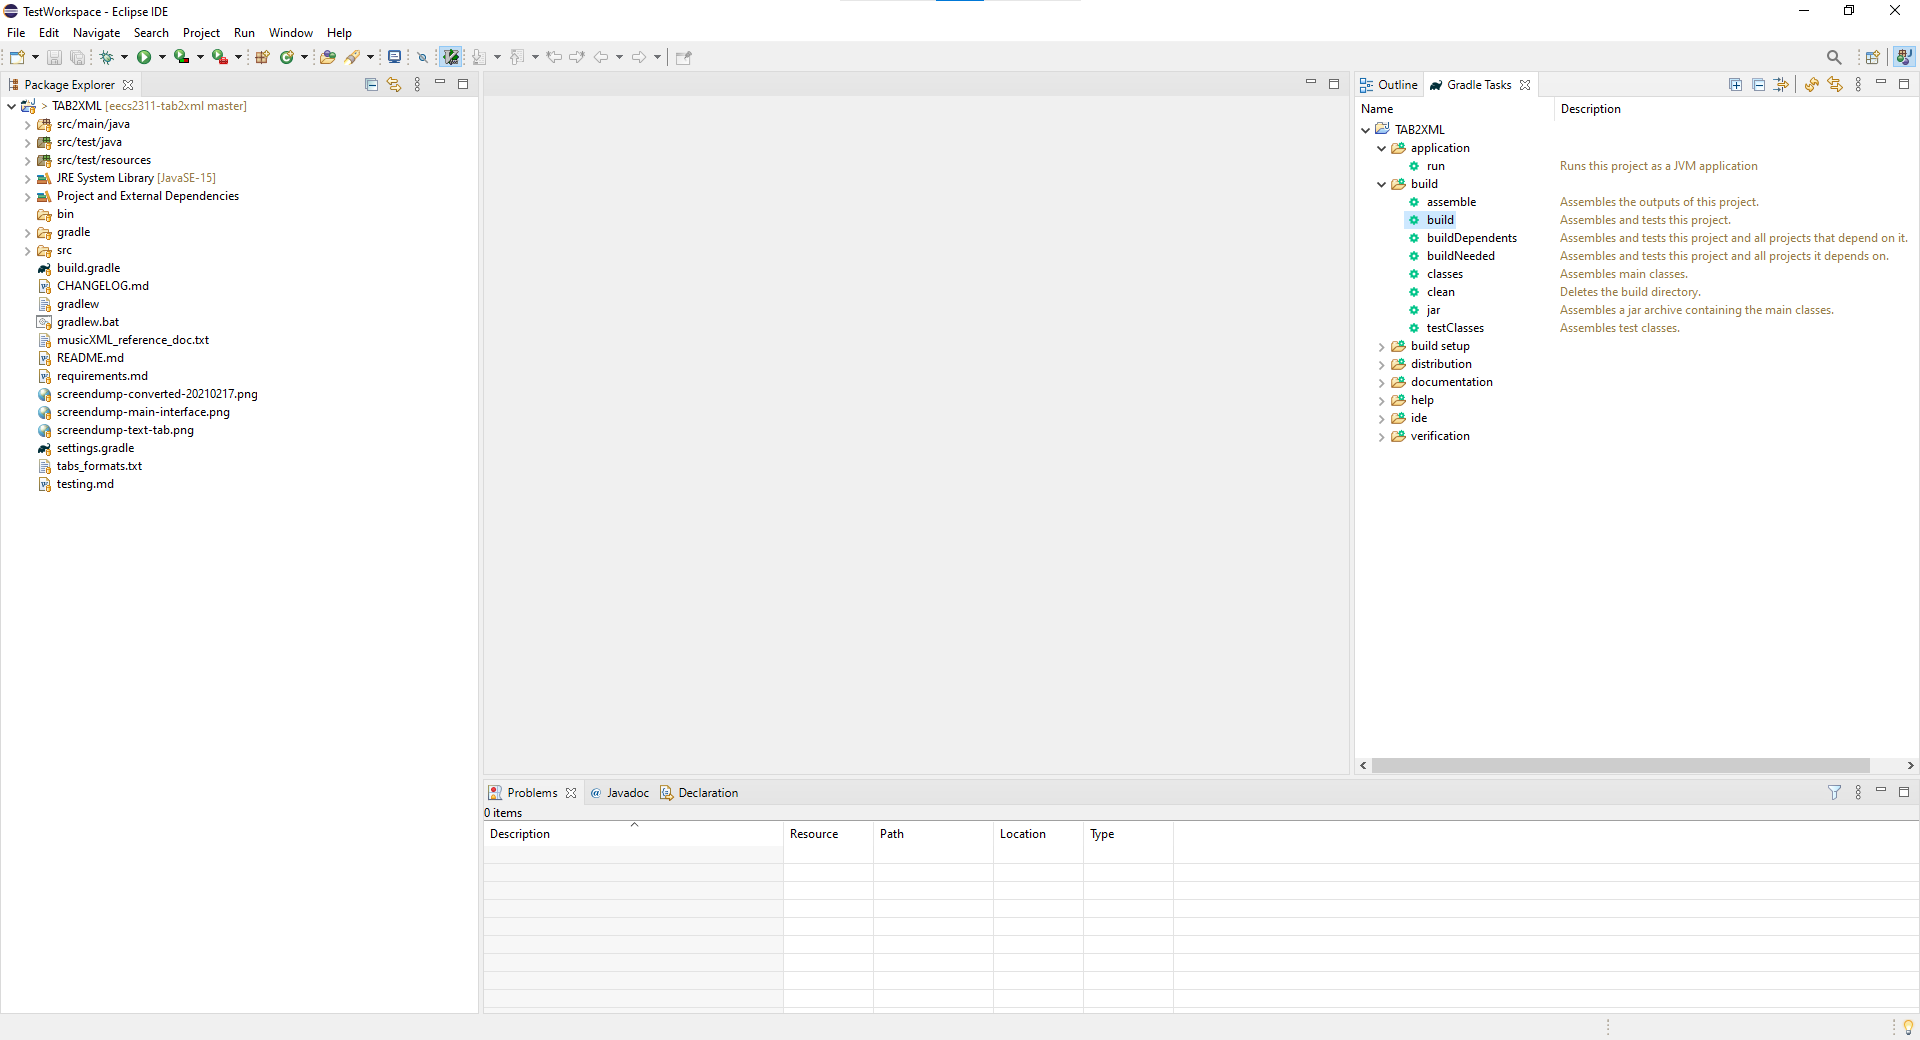
\includegraphics[width=.9\linewidth]{../Screenshots/eclipse-build.png}
\end{center}
\end{enumerate}
\subsection{Commandline}
\label{sec:org5dc0870}
\begin{enumerate}
\item Use the command \texttt{git clone https://github.com/ahopk127/eecs2311-tab2xml.git} to clone the project to the directory of your choice
\item Change directory to the directory where you installed the project, then use Gradle (\texttt{./gradlew build}, if that doesn't work try running \texttt{chmod +x ./gradlew} then \texttt{./gradlew build}) to build the project.
\end{enumerate}
\newpage

\section{How to Use TAB2XML}
\label{sec:orgb3ef593}
\subsection{Convert Text Tab}
\label{sec:org194ba17}
\begin{enumerate}
\item Run the application.  In Eclipse, double-click the green "run" item in the "application" folder.  In commandline, use the command \texttt{./gradlew run} in the program directory.\\
You should see a window like this:
\begin{center}
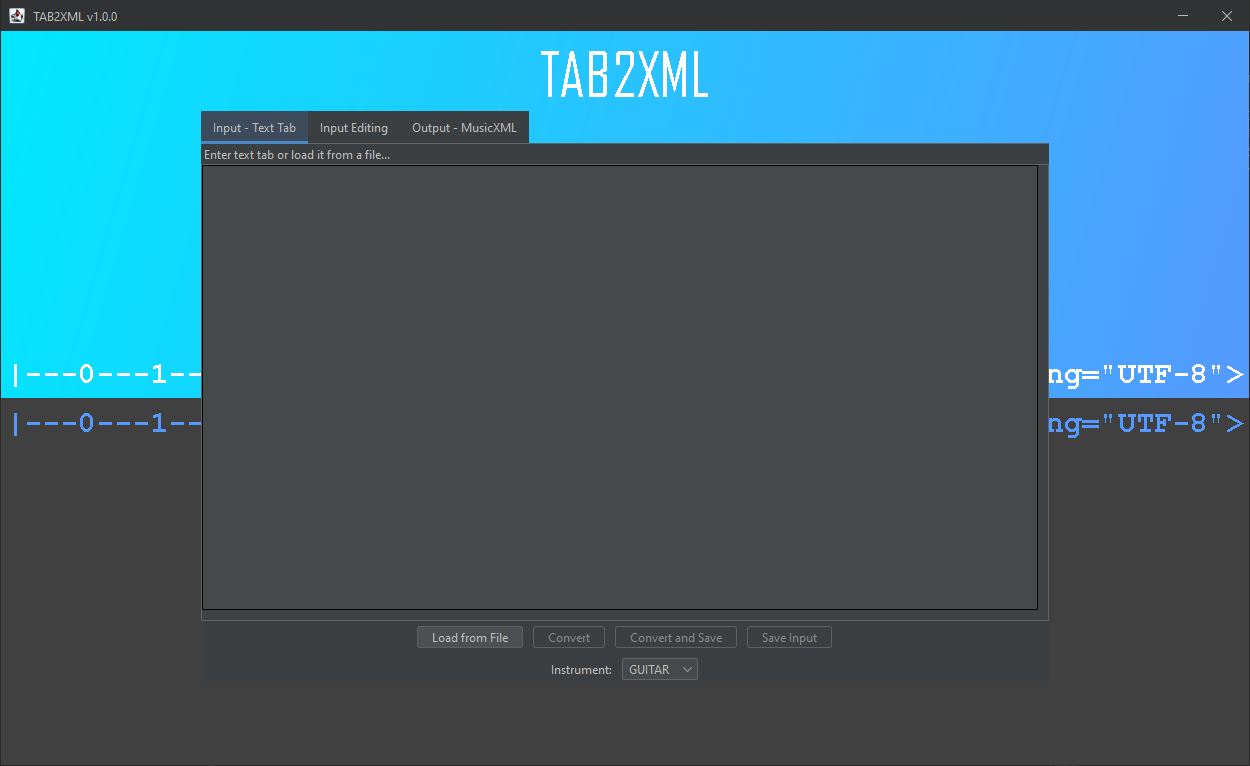
\includegraphics[width=.9\linewidth]{../Screenshots/main-interface-tabbedview-1.0.0.png}
\end{center}
\item Input your text tab into the application.  There are multiple ways of doing this:
\begin{itemize}
\item Type or copy-and-paste your text tab into the text box.
\item Press the "Load from File" button then choose a file to load your text tab from a file.
\item Drag and drop a text tab file into the input box
\item Drag and drop text into the input box
\end{itemize}
\begin{center}
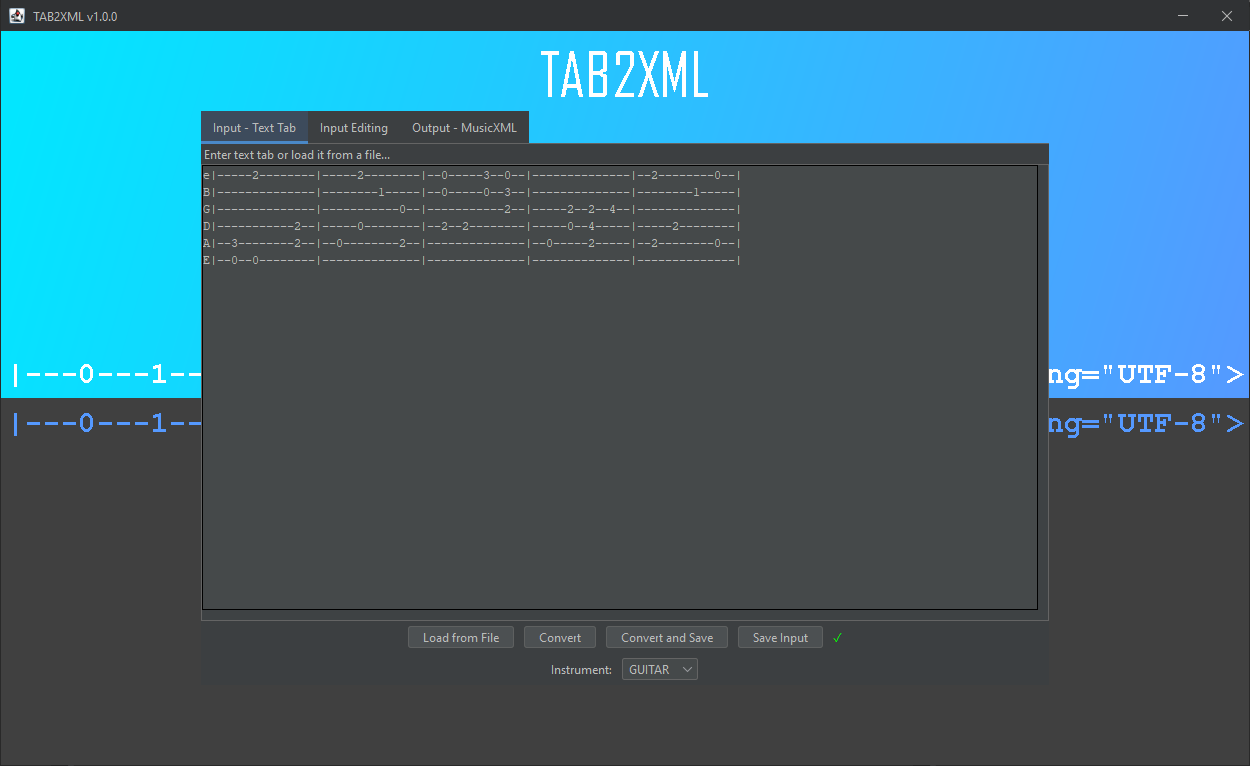
\includegraphics[width=.9\linewidth]{../Screenshots/sample-inputs-tabbedview-1.0.0.png}
\end{center}
\item Press the "Convert" button.  The text tab will be replaced with the corresponding MusicXML.
\begin{center}
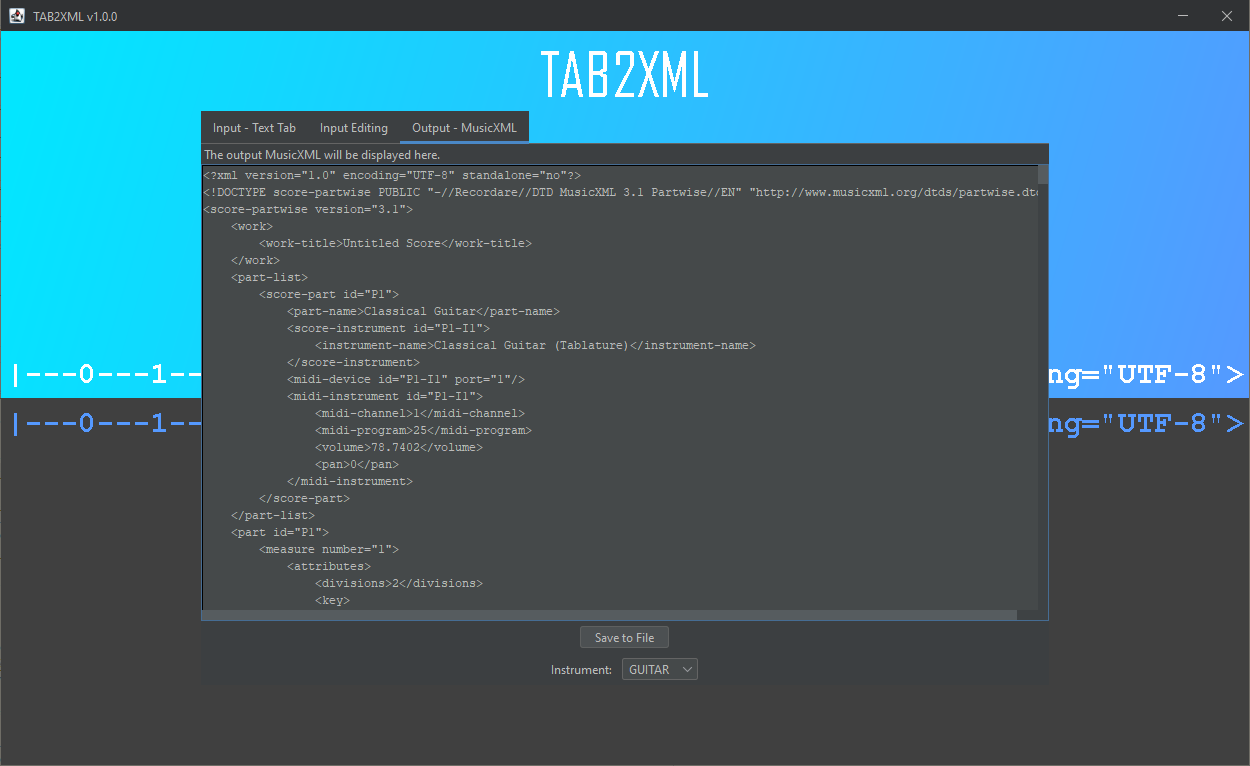
\includegraphics[width=.9\linewidth]{../Screenshots/converted-20210413-tabbedview.png}
\end{center}
\item You can now copy-and-paste the MusicXML, or save it to a file using the "Save to File" button. \\
Here is a screenshot of the produced MusicXML, rendered using \href{https://musescore.org/en/download}{MuseScore 3.6.2}:
\begin{center}
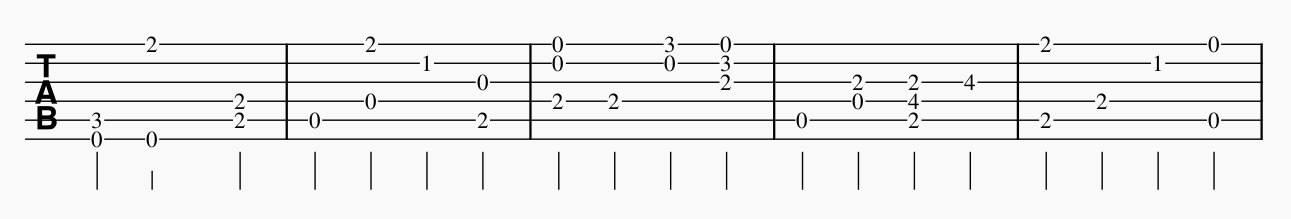
\includegraphics[width=.9\linewidth]{../Screenshots/converted-20210413-musescore.png}
\end{center}
\end{enumerate}
\subsection{Editing Text Tabs}
\label{sec:orgf3e4430}
After converting text tab with the "Convert" button, you can switch to the "Input" tab to edit the input text tab.  Use "Save Input" to save the (edited) input to a file.

You can use the "Input Editing" tab for more precise editing of the input.  This view also allows you to set metadata such as the title of the output score.  The view should look like this:
\begin{center}
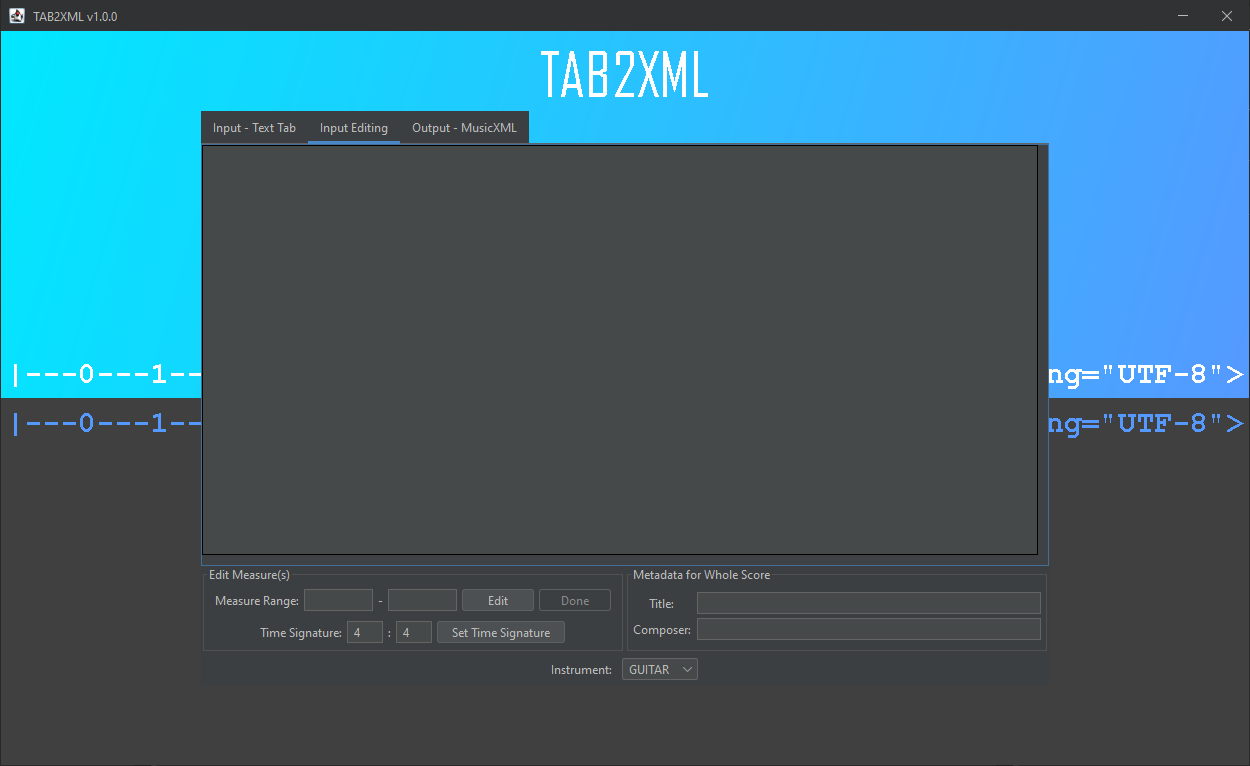
\includegraphics[width=.9\linewidth]{../Screenshots/input-editing-tabbedview-1.0.0.png}
\end{center}
\subsubsection{Editing Measures}
\label{sec:org9754a6a}
One thing you can do with this editing view is editing a single measure or a range of measures from the input tablature.  To do this, follow the following steps:
\begin{enumerate}
\item Input your text tablature in the "Input" tab if it isn't already there.
\item Navigate to the "Input Editing" tab.
\item Input the desired range of measures in the "Measure Range" boxes on the bottom left.
\item Press the "Edit" button.  You should see something like this:
\begin{center}
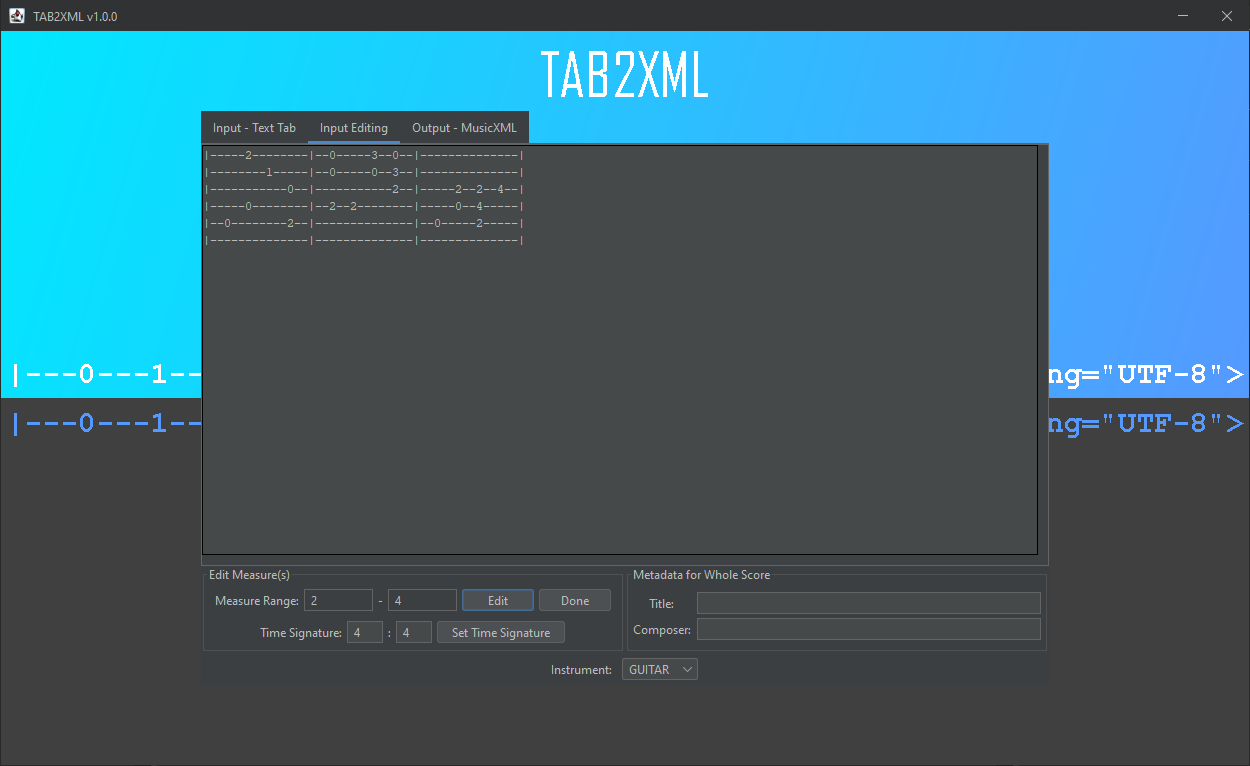
\includegraphics[width=.9\linewidth]{../Screenshots/sample-input-editing-tabbedview.png}
\end{center}
\item Edit the tablature in the text box, then click "Done".
\end{enumerate}

Note: This system is not as sophisticated as the parser, and can occasionally fail when exposed to tabs with complex "decorations" that aren't part of the measure text.  If this system fails, try removing decorations then trying again. \\
\textbf{Warning}: Editing a measure region then saving it will remove any decorations from the tab.
\subsubsection{Editing Metadata}
\label{sec:org912d58d}
You can also use the Input Editing tab to edit metadata.  To edit the title and/or composer, simply enter them into the text boxes on the bottom right.  There is no need to press any "Edit" or "Save" buttons, they will simply be entered in the score when it is converted.

Editing the time signature of a measure range is a bit more complicated:
\begin{enumerate}
\item Select the measure range as if you were editing it (follow \hyperref[sec:org9754a6a]{these steps} up to step 4).
\item Input the time signature in the text boxes on the bottom-left.
\item Press the "Set Time Signature" button.
\end{enumerate}

Note: If no time signature range was selected, the "Set Time Signature" button will still work - it will ask you if you want to set the time signature for the whole score.
\subsection{Other Use Cases}
\label{sec:org9ea4071}
\begin{itemize}
\item You can use the "Convert and Save" button to convert a text tab and save it to a file in one step.
\item To clear the text box, press Ctrl-A then Delete.  If you want to load in another text tab, you don't need to do this.  Simply press "Load from File" or drag and drop to load another text tab.
\end{itemize}
\subsection{How to Use in Code}
\label{sec:orge38ddb3}
If you would like to use this project in your own program, the following code can be used to convert tab to MusicXML:

\begin{verbatim}
tab2xml.parser.Parser parser = new tab2xml.parser.Parser(INPUT, INSTRUMENT);  
String output = parser.parse();  
\end{verbatim}

Notes:
\begin{itemize}
\item INPUT is the text tab.  It should be a \texttt{String} containing the contents of the tablature, not a file or a filepath.
\item INSTRUMENT is the instrument the tab is for.  It should be an instance of \texttt{tab2xml.parser.Instrument}.
\item You will need to add a try-catch statement to handle the checked exceptions thrown by \texttt{Parser.parse()}.
\end{itemize}

\section{Supported Tabs}
\label{sec:orgc99a726}
You can find a sample of supported tabs \href{https://github.com/ahopk127/eecs2311-tab2xml/tree/develop/src/test/resources/test-tabs}{here}.
\subsection{Guitar/Bass}
\label{sec:orgda7baa8}
\subsubsection{supported features}
\label{sec:org3a28e89}
\begin{enumerate}
\item hammer-on notations
\item pull-off notations
\item grace notes
\item repeated measures
\item hammer-on/pull-off combination sequences
\item chords
\item in-line comments
\item multiline comments
\end{enumerate}

\subsection{Drum}
\label{sec:orgdef6f11}
\subsubsection{supported drum types notation}
\label{sec:org9e16c60}
\begin{enumerate}
\item \texttt{BD} - Bass Drum 1
\item \texttt{Bd} - Bass Drum 2
\item \texttt{SS} - Side Stick
\item \texttt{SD} - Snare
\item \texttt{ES} - Electric Snare
\item \texttt{FT} - Low Floor Tom
\item \texttt{HH} - Closed Hi-Hat
\item \texttt{Ft} - High Floor Tom
\item \texttt{PH} - Pedal Hi-Hat
\item \texttt{LT} - Low Tom
\item \texttt{OH} - Open Hi-Hat
\item \texttt{LM} - Low-Mid Tom
\item \texttt{MT} - Hi-Mid Tom
\item \texttt{CC} - Crash Cymbal 1
\item \texttt{HT} - High Tom
\item \texttt{RD} - Ride Cymbal 1
\item \texttt{Ch} - Chinese Cymbal
\item \texttt{RB} - Ride Bell
\item \texttt{TA} - Tambourine
\item \texttt{SC} - Splash Cymbal
\item \texttt{CB} - Cowbell
\item \texttt{Cc} - Crash Cymbal 2
\item \texttt{Rd} - Ride Cymbal 2
\item \texttt{HC} - Open Hi Conga
\item \texttt{LC} - Low Conga
\end{enumerate}
\end{document}
